\section{Model predictions errors for Vietnam and the United States}

This section presents the results obtained from the different versions of the model when trained with data for Vietnam and the \gls{US}.
\autoref{fig:predictions-vietnam-baseline} and \autoref{fig:predictions-usa-baseline} present the predictions made by the baseline model.
\autoref{fig:predictions-vietnam-fb1} and \autoref{fig:predictions-usa-fb1} present the predictions made by the model's versions that included Facebook's Movement Range Maps dataset to inform the model about the contact rate.

% ERRORS

\begin{table}[!htb]
    \centering
    \begin{tabular}{| c | c | c | c | c | c | c| c |}
        \multirow{2}{*}{Days}
            & \multirow{2}{*}{Loc.}
            & \multicolumn{3}{c |}{Baseline}
            & \multicolumn{3}{c |}{2nd. Ver} \\ \cline{3-8}
            & & MAE & MAPE & RMSE & MAE & MAPE & RMSE \\ \hline\hline

        \multirow{2}{*}{7}
            & VN & 2.409 & 4.033 & 2.470 & \textbf{2.356} & \textbf{3.943} & \textbf{2.420} \\ \cline{2-8}
            & US & \textbf{727.905} & \textbf{0.116} & \textbf{834.818} & 826.050 & 0.132 & 949.121 \\ \hline

        \multirow{2}{*}{14}
            & VN & 2.222 & 3.549 & 2.321 & \textbf{2.221} & \textbf{3.540} & \textbf{2.310} \\ \cline{2-8}
            & US & \textbf{1689.681} & \textbf{0.267} & \textbf{2022.840} & 1871.675 & 0.296 & 2225.024 \\ \hline

        \multirow{2}{*}{21}
            & VN & 1.743 & 2.697 & 1.969 & \textbf{1.676} & \textbf{2.609} & \textbf{1.929} \\ \cline{2-8}
            & US & \textbf{2986.879} & \textbf{0.467} & \textbf{3662.566} & 3155.909 & 0.494 & 3803.063 \\ \hline

        \multirow{2}{*}{28}
            & VN & 3.530 & 4.318 & 5.408 & \textbf{3.301} & \textbf{4.062} & \textbf{5.074} \\ \cline{2-8}
            & US & 4512.893 & 0.697 & 5576.519 & \textbf{4495.416} & \textbf{0.695} & \textbf{5401.567} \\ \hline
    \end{tabular}
    \caption{Out-of-sample errors of the model's predictions on the number of deaths for Vietnam and the United States. The lowest errors for each evaluation metrics at each location are highlighted.}
\end{table}

\begin{table}[!htb]
    \centering
    \begin{tabular}{| c | c | c | c | c | c | c| c |}
        \multirow{2}{*}{Days}
            & \multirow{2}{*}{Loc.}
            & \multicolumn{3}{c |}{Baseline}
            & \multicolumn{3}{c |}{2nd. Version} \\ \cline{3-8}
            & & MAE & MAPE & RMSE & MAE & MAPE & RMSE \\ \hline\hline

        \multirow{2}{*}{7}
            & VN & 96.166 & 27.928 & 106.205 & \textbf{88.005} & \textbf{25.491} & \textbf{97.969} \\ \cline{2-8}
            & US & \textbf{2006.080} & \textbf{1.343} & \textbf{2415.311} & 2051.455 & 1.370 & 2976.705 \\ \hline

        \multirow{2}{*}{14}
            & VN & 110.478 & 32.456 & 117.440 & \textbf{99.469} & \textbf{29.140} & \textbf{106.410} \\ \cline{2-8}
            & US & 6775.296 & 4.326 & 8842.444 & \textbf{6004.020} & \textbf{3.849} & \textbf{7582.764} \\ \hline

        \multirow{2}{*}{21}
            & VN & 174.686 & 41.840 & 207.332 & \textbf{161.454} & \textbf{38.390} & \textbf{194.470} \\ \cline{2-8}
            & US & 12426.818 & 7.766 & 16039.493 & \textbf{10781.952} & \textbf{6.974} & \textbf{14765.447} \\ \hline

        \multirow{2}{*}{28}
            & VN & 357.254 & 52.338 & 502.876 & \textbf{342.409} & \textbf{49.266} & \textbf{490.063} \\ \cline{2-8}
            & US & 16943.424 & \textbf{10.771} & \textbf{21371.281} & \textbf{16516.025} & 10.859 & 21514.390 \\ \hline
    \end{tabular}
    \caption{Out-of-sample errors of the model's predictions on the number of new cases for Vietnam and the United States. The lowest errors for each evaluation metrics at each location are highlighted.}
\end{table}

\begin{table}[!htb]
    \centering
    \begin{tabular}{| c | c | c | c | c | c | c| c |}
        \multirow{2}{*}{Days}
            & \multirow{2}{*}{Loc}
            & \multicolumn{3}{c |}{Baseline}
            & \multicolumn{3}{c |}{2nd. Version} \\ \cline{3-8}
            & & MAE & MAPE & RMSE & MAE & MAPE & RMSE \\
        \hline\hline

        \multirow{2}{*}{7}
            & VN & \textbf{234.690} & \textbf{2.022} & \textbf{312.078} & 241.284 & 2.081 & 313.870 \\ \cline{2-8}
            & US & \textbf{39553.840} & \textbf{0.106} & \textbf{39745.361} & 61863.751 & 0.166 & 62287.404 \\ \hline

        \multirow{2}{*}{14}
            & VN & 672.504 & 5.098 & 831.731 & \textbf{643.697} & \textbf{4.894} & \textbf{785.383} \\ \cline{2-8}
            & US & \textbf{30561.907} & \textbf{0.081} & \textbf{33712.852} & 88894.016 & 0.233 & 94595.820 \\ \hline

        \multirow{2}{*}{21}
            & VN & 1285.683 & 8.495 & 1645.257 & \textbf{1206.696} & \textbf{7.994} & \textbf{1533.632} \\ \cline{2-8}
            & US & \textbf{71921.579} & \textbf{0.184} & \textbf{97776.403} & 132684.773 & 0.341 & 151150.555 \\ \hline

        \multirow{2}{*}{28}
            & VN & 2650.472 & 14.012 & 3786.242 & \textbf{2512.913} & \textbf{13.276} & \textbf{3605.530} \\ \cline{2-8}
            & US & \textbf{137006.424} & \textbf{0.342} & \textbf{189405.400} & 210325.947 & 0.529 & 259678.415 \\ \hline
    \end{tabular}
    \caption{Out-of-sample errors of the model's predictions on the number of cumulative cases for Vietnam and the United States. The lowest errors for each evaluation metrics at each location are highlighted.}
\end{table}

\subsection{Reproduction number and fatality rate}

\begin{figure}[!htb]
    \centering

    \begin{subfigure}[b]{\linewidth}
        \centering
        \begin{subfigure}[b]{0.4\linewidth}
            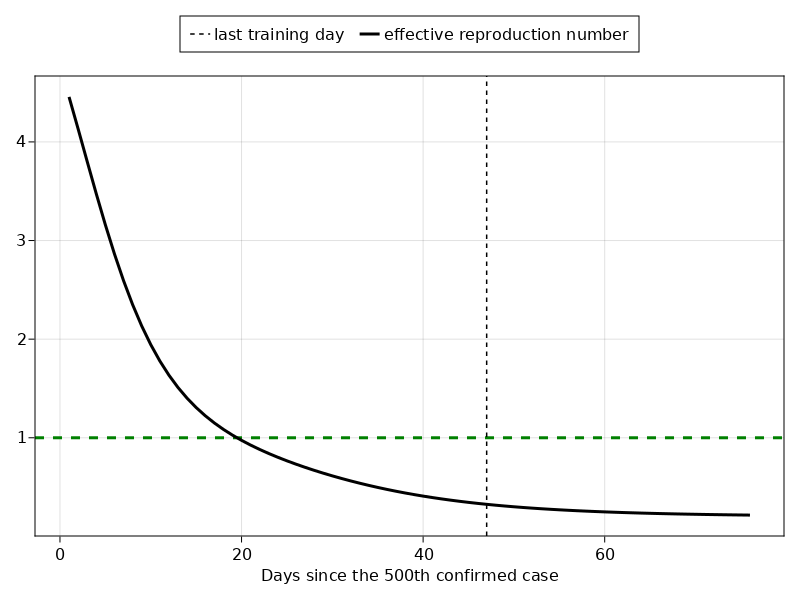
\includegraphics[width=\linewidth]{baseline/vietnam/20211216111951.baseline.vietnam.R_effective.png}
        \end{subfigure}
        \begin{subfigure}[b]{0.4\linewidth}
            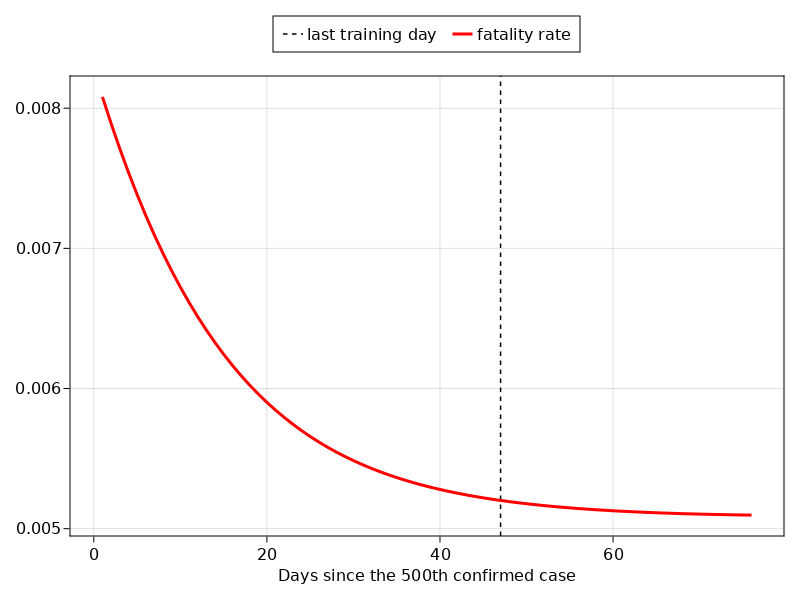
\includegraphics[width=\linewidth]{baseline/vietnam/20211216111951.baseline.vietnam.fatality_rate.png}
        \end{subfigure}
        \subcaption{Baseline model}
    \end{subfigure}

    \begin{subfigure}[b]{\linewidth}
        \centering
        \begin{subfigure}[b]{0.4\linewidth}
            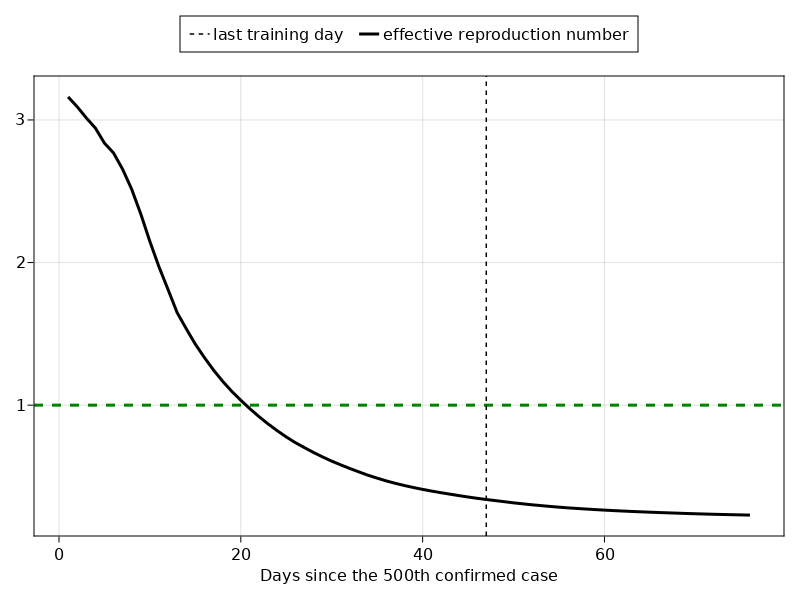
\includegraphics[width=\linewidth]{fb1/vietnam/20211216231719.fbmobility1.vietnam.R_effective.png}
        \end{subfigure}
        \begin{subfigure}[b]{0.4\linewidth}
            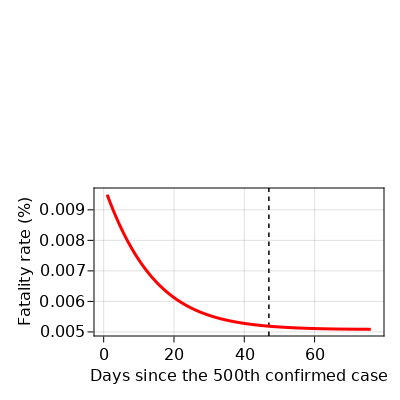
\includegraphics[width=\linewidth]{fb1/vietnam/20211216231719.fbmobility1.vietnam.fatality_rate.png}
        \end{subfigure}
        \subcaption{2nd. version}
    \end{subfigure}

    \caption{The effective reproduction number and the fatality rate for Vietnam learned by different versions of the model}
    \label{fig:R0-and-fatality-vietnam}
\end{figure}

\begin{figure}[!htb]
    \centering

    \begin{subfigure}[b]{\linewidth}
        \centering
        \begin{subfigure}[b]{0.4\linewidth}
            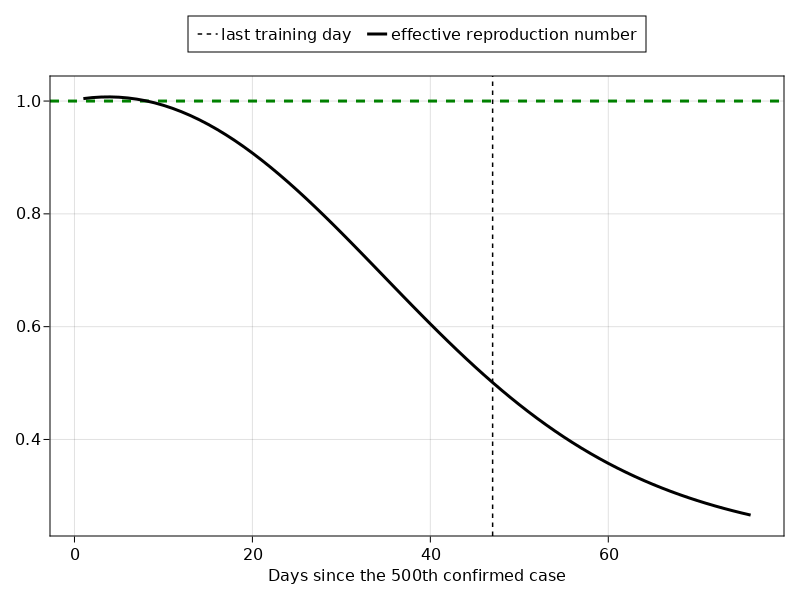
\includegraphics[width=\linewidth]{baseline/unitedstates/20211216125000.baseline.unitedstates.R_effective.png}
        \end{subfigure}
        \begin{subfigure}[b]{0.4\linewidth}
            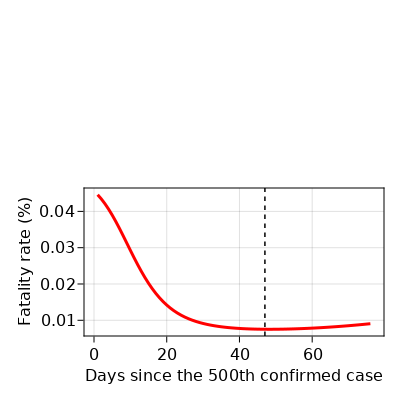
\includegraphics[width=\linewidth]{baseline/unitedstates/20211216125000.baseline.unitedstates.fatality_rate.png}
        \end{subfigure}
        \subcaption{Baseline model}
    \end{subfigure}

    \begin{subfigure}[b]{\linewidth}
        \centering
        \begin{subfigure}[b]{0.4\linewidth}
            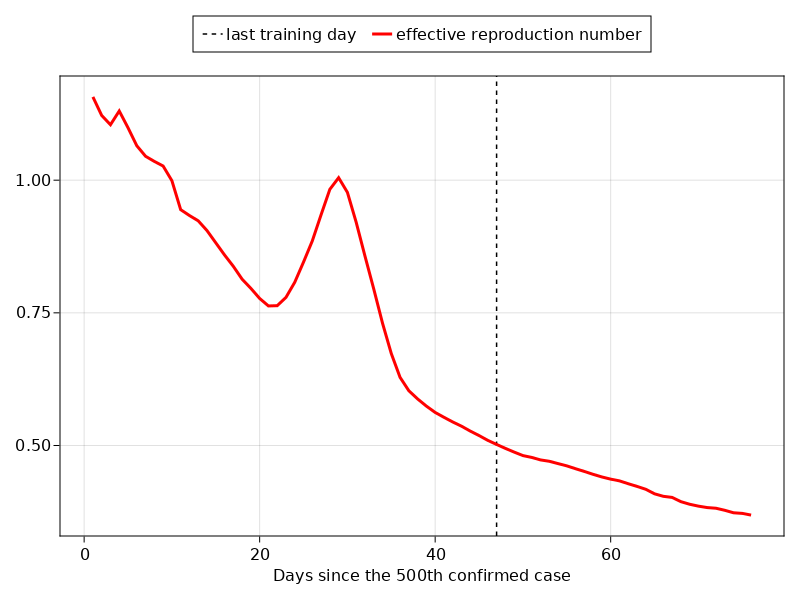
\includegraphics[width=\linewidth]{fb1/unitedstates/20211216233634.fbmobility1.unitedstates.R_effective.png}
        \end{subfigure}
        \begin{subfigure}[b]{0.4\linewidth}
            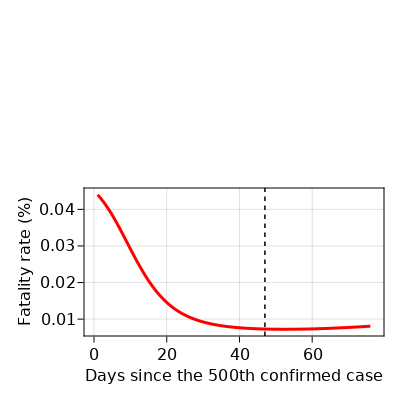
\includegraphics[width=\linewidth]{fb1/unitedstates/20211216233634.fbmobility1.unitedstates.fatality_rate.png}
        \end{subfigure}
        \subcaption{2nd. version}
    \end{subfigure}

    \caption{The effective reproduction number and the fatality rate for the United States learned by different versions of the model}
    \label{fig:R0-and-fatality-usa}
\end{figure}
